\documentclass[aspectratio=169]{beamer}
\usepackage[utf8]{inputenc}
\usepackage{tikz}

\usetheme{Rochester}
\beamertemplatenavigationsymbolsempty

\usetikzlibrary{shapes}
\usetikzlibrary{shapes.multipart}

\title{Querying Linked Data with SPARQL and the Wikidata Query Service}
\author{Lucas Werkmeister}
\date{2019-12-27}

\begin{document}

\frame{\titlepage}

\begin{frame}[fragile]
  \frametitle{An example graph}
  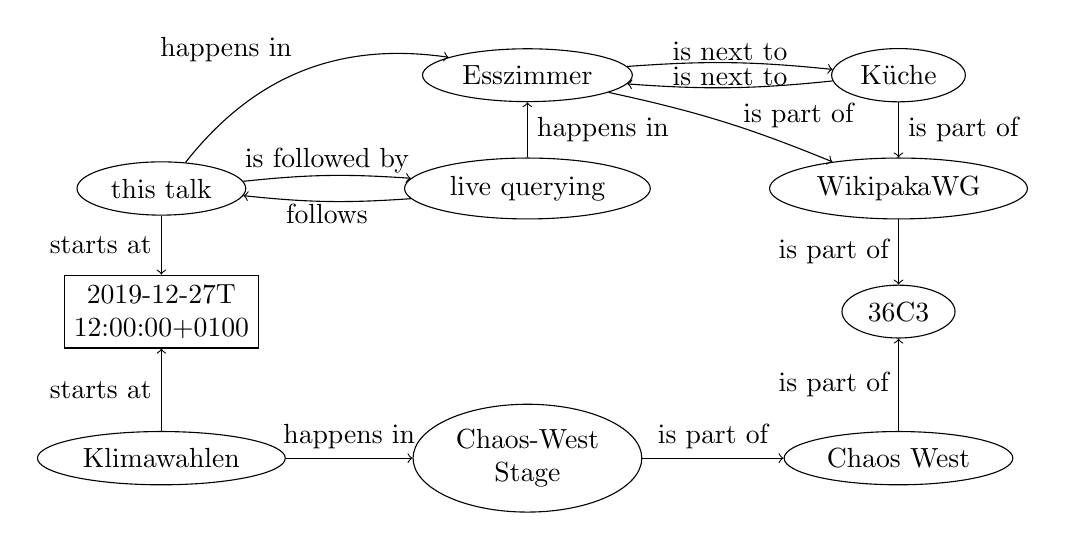
\begin{tikzpicture}[
      iri/.style={ellipse,draw},
      literal/.style={rectangle,draw},
      predicate/.style={->,auto},
      predicate bidi/.style={predicate,bend left=5,inner sep=0.25mm},
      every text node part/.style={align=center},
    ]
    \matrix[row sep=7mm,column sep=15mm] {
      & \node[iri] (Esszimmer) {Esszimmer}; & \node[iri] (Kueche) {Küche}; \\
      \node[iri] (this talk) {this talk}; & \node[iri] (live querying) {live querying}; & \node[iri] (WikipakaWG) {WikipakaWG}; \\
      \node[literal] (Tag 1 noon) {2019-12-27T\\12:00:00+0100}; & & \node[iri] (36C3) {36C3}; \\
      \node[iri] (Klimawahlen) {Klimawahlen}; & \node[iri] (Chaos-West Stage) {Chaos-West\\Stage}; & \node[iri] (Chaos West) {Chaos West}; \\
    };
    \draw[predicate bidi] (this talk) to node {is followed by} (live querying);
    \draw[predicate bidi] (live querying) to node {follows} (this talk);
    \draw[predicate,bend left] (this talk) to node {happens in} (Esszimmer);
    \draw[predicate,swap] (live querying) to node {happens in} (Esszimmer);
    \draw[predicate bidi] (Esszimmer) to node {is next to} (Kueche);
    \draw[predicate bidi,swap] (Kueche) to node {is next to} (Esszimmer);
    \draw[predicate,bend left=5] (Esszimmer) to node [pos=.6,inner sep=0] {is part of} (WikipakaWG);
    \draw[predicate] (Kueche) to node {is part of} (WikipakaWG);
    \draw[predicate,swap] (WikipakaWG) to node {is part of} (36C3);
    \draw[predicate,swap] (this talk) to node {starts at} (Tag 1 noon);
    \draw[predicate] (Klimawahlen) to node {starts at} (Tag 1 noon);
    \draw[predicate] (Klimawahlen) to node {happens in} (Chaos-West Stage);
    \draw[predicate] (Chaos-West Stage) to node {is part of} (Chaos West);
    \draw[predicate] (Chaos West) to node {is part of} (36C3);
  \end{tikzpicture}
\end{frame}

\end{document}
